%!TEX root = ../main.tex

%!TEX root = ../main.tex


\chapter{Rule Learning Guided by External Sources}
\label{sec:framework}
%---------------------------------------------------------%

In this chapter, we introduce our framework for rule learning guided by external sources,
discuss challenges associated with it, and finally propose its concrete instantiation with embedding models.

%\section{Background}
%%---------------------------------------------------------%
%
%We assume countable sets $\mathcal{R}$ of unary and binary relation names and $\mathcal{C}$  of constants. 
%A \emph{knowledge graph} (KG) $\G$ is a finite set of ground atoms $a$ of the form
%$P(b,c)$ and $C(b)$ over %the 
%$\R\cup\C$.
%With $\Sigma_{\cG}$, the \emph{signature} of $\G$, we denote elements of $\R\cup\C$ that occur in $\G$.\looseness=-1
%
%
%We define rules over KGs following the standard approach of non-monotonic logic programs under the answer set semantics %, see e.g. 
%\cite{GL1988}.
%Let $\X$ be a countable set of variables.
%A \emph{rule} $r$ is %an expression 
%of the form
%$
%\mi{head \leftarrow body},
%$
%where $\mi{head}$, or $\mi{head}(r)$, is an atom 
%%of the form $a(\vec{X})$ 
%over $\R\cup\C\cup\X$ 
%%and $\vec{X}$ are its variables,
%and $body$, or $\mi{body}(r)$, is a conjunction of positive and negative atoms 
%over $\R\cup\C\cup\X$.
%Finally, 
%$\mi{body^+(r)}$ and $\mi{body^-(r)}$ denote the atoms that occur in $\mi{body(r)}$ positively and negatively respectively, that is, the rule can be written as
%$
%\mi{head(r) \leftarrow body^+(r), not\ body^-(r)}.
%$
%A rule is \emph{Horn}, if all head variables occur in the body,
%and $\mi{body^-(r)}$ is empty.
%
%
%We define \emph{execution} of rules with default negation~\cite{GL1988} over KGs in the standard way.
%More precisely, let $\G$ be a KG, $r$ a rule over $\Sigma_\G$, 
%and $a$ be an atom over $\Sigma_\G$.
%Then, $r \models_\G a$ holds if there is a variable assignment that maps atoms $\mi{body^+(r)}$ in $\G$ such that it does not map any of the atoms in $\mi{body^-(r)}$ in $\G$. 
%Then, let $\G_r = \G \cup \set{a \mid r \models_\G a}$. 
%Intuitively, $\G_r$ extends $\G$ with edges derived from $\G$ by applying $r$.

\section{Problem Statement and Proposal of General Solution} 
%---------------------------------------------------------%
Let $\G$ be a KG over the signature $\Sigma_{\G}=\tuple{\cR_\G,\cC_\G}$. 
A \emph{probabilistic KG} $\PG$ is a pair $\PG = (\G,f)$ 
where $f:\cR_\G\times \cC_\G \times \cC_\G\rightarrow [0,1]$ is a probability function over the facts over $\Sigma_{\G}$ such that for each atom $a \in \G $ it holds that $f(a) = 1$.

The goal of our work is to learn rules that not only describe the available graph $\cG$ well, but also predict highly probable facts based on the function $f$.
The key questions now are how to define the quality of a given rule $r$ based on $\PG$ and how to exploit this quality during rule learning for pruning out not promising rules. 

% Let $\G_r = \G \cup \set{a \mid r \models_\G a}$, where $r$ is a rule mined from $\G$.
% Intuitively, $\G_r$ extends $\G$ with edges derived from $\G$ by applying $r$.
% The set $\G_r \setminus \G$ denotes all facts that may be present
% in the %real
% ideal KG, but are missing in the incomplete $\G$, and $f$ gives the probability of these facts.

A quality measure $\mu$ for rules over probabilistic KGs 
is a function $\mu: (r,\PG) \mapsto \alpha$, where $\alpha \in  [0,1]$.
In order to measure the quality $\mu$ of $r$ over $\PG$ we propose: 
\begin{itemize}
\item 
to measure the quality $\mu_1$ of $r$ over $\G$, where $\mu_1: (r,\cG) \mapsto \alpha \in  [0,1]$,
\item
to measure the quality $\mu_2$ of $\G_r$ by relying on $\PG_r=(\cG_r,f)$, 
where $\mu_2{:}\, (\G'{,}\, (\G,f)) \mapsto  \alpha \,{\in}\, [0,1]$ for $\G' \supseteq \G$ is the quality of extensions $\G'$ of $\G$ over $\Sigma_\G$ given $f$,
and 
\item
to combine the result as the weighted sum.
\end{itemize}
That is, we define our hybrid rule quality function $\mu(r,\PG)$ as follows:
\begin{align}\label{eq:hm}
	\mu(r,\PG)= (1 - \lambda)\times \mu_1(r,\cG) + \lambda \times \mu_2(\G_r,\PG).
\end{align}
In this formula $\mu_1$ can be any classical quality measure of rules over complete graphs. %  and 
% $\mu_2$ 
% \thi{mu2 what?}.
Intuitively, $\mu_2(\G_r,\PG)$ is the quality of $\G_r$ wrt $f$ that allows us to capture the information about facts missing in $\G$ that are relevant for $r$.
The weighting factor %parameter 
$\lambda$, we call it \textit{embedding weight}, allows one to choose whether %one prefers 
to rely more on the classical measure $\mu_1$ or on the measure $\mu_2$ of the quality of the facts that 
are predicted by $r$ over $\G$.

\subsection{Challenges} 
%---------------------------------------%
There are several challenges that one has to face when realizing our approach:
\begin{itemize}
\item First, given an incomplete KG $\G$, one has to define $f$
such that $(\G,f)$ satisfies the expectations, i.e., reflects well the probabilities of missing facts.
\item Second, one has to define $\mu_1$ and $\mu_2$ that also satisfy the expectations and admit efficient implementation.
\item Third, the adaptation of existing rule learning approaches to account for the probabilistic function $f$ without the loss of scalability is not trivial. 
Indeed, materializing $f$ by augmenting $\cG$ with all possible probabilistic facts over $\Sigma_{\cG}$ and subsequently applying standard rule learning methods on the obtained graph is not practical. Storing such potentially enormous augmented graph 
where many probabilistic facts are irrelevant for the extraction of meaningful rules might be simply infeasible.
\end{itemize}
%\looseness=-1
\section{Realization of General Solution}
\label{section: realisation}
%------------------------------------------------------------%
We now %present 
describe how we addressed the above stated challenges in this thesis.
In Section~\ref{section: realisation} we present concrete realizations of $f$, $\mu_1$ and $\mu_2$, and in Section~\ref{sec:sys} we discuss how we implemented them and adapted within an %rule learning as an 
end-to-end rule learning system.

% In what follows we present our solution to the above challenges by discussing the realizations of $f$, $\mu_1$ and $\mu_2$, and in Section~\ref{sec:sys} present the end-to-end rule learning systems that exploits our proposals.

\subsection{Realization of the Probabilistic Function $f$}
%------------------------------------------------------------%
We propose to define $f$ by relying on embeddings of KGs.
Embedding models can be used to estimate the likelihood of potentially missing binary atoms
using a scoring function $\mi{\xi: \cR_\cG \times \cC_\cG \times \cC_\cG \rightarrow \mathbb{R}}$.
Examples of concrete scoring functions can be found, e.g., in~\cite{DBLP:journals/tkde/WangMWG17}.
Since embeddings per se are not in the focus of this thesis,
we will not give further details on them and refer the reader to~\cite{DBLP:journals/tkde/WangMWG17} for an overview.
Note that our framework is not dependent on a concrete embedding model. 
What is important for us is that embeddings can be used to construct probabilistic representations~\cite{DBLP:conf/aaai/NickelRP16} of atoms missing in KGs and we use this to define $f$.

Consider an auxiliary definition. Given a KG $\G$, and an atom $a=p(s,o)$, the set $\G_s$ consists of $a$ and all atoms $a'$ that are obtained from $a$ by replacing $s$ with a constant from $\Sigma_\G$, except for those that are already in $\G$. 
Then, given a scoring function $\xi$, $[\G_s]$ is a list of atoms from $\G_s$ ordered in the descending order.
Finally, the \emph{subject rank}~\cite{DBLP:journals/corr/abs-1301-3485} of $a$ given $\xi$, $\mi{subject\_rank_\xi(a)}$ is the position of $a$ in $[\G_s]$. 
Analogously one can define $[\G_o]$ and the corresponding 
\emph{object rank}~\cite{DBLP:journals/corr/abs-1301-3485} of $a$ given $\xi$, that is, $\mi{object\_rank_\xi(a)}$. 

Now we are ready to define the function $f$ for an atom $a$ %:it i
as the average of its subject and object inverted ranks given $\xi$~\cite{DBLP:journals/corr/abs-1301-3485}, i.e.:
\begin{align}
\label{eq:f}
\mi{f_\xi(a)} = 0.5\times(1/\mi{subject\_rank_\xi(a)}+ 1/\mi{object\_rank_\xi(a)})
\end{align}



\subsection{Realization of $\mu_1$}
%---------------------------------------------------%
This measure should reflect the descriptive quality of a given rule $r$ with respect to $\cG$.
There are many classical data mining measures that can be used as $\mu_1$, see, e.g. \cite{DBLP:conf/eurogp/MinhdNT18,amie,carl,measureskg} for $\mu_1$s proposed specifically for KGs. In principle, we should choose a suitable measure that correctly describes the KG.

In our work we selected the following two measures for $\mu_1$:
\emph{standard confidence} and \emph{PCA confidence}. While standard confidence of a rule is the conditional probability of rule's head given its body, computed based on closed world assumption (CWA), PCA confidence is its generalisation to the open world assumption (OWA), which does not penalize rules that predict facts $p(s,o)$, such that $p(s,o')\not \in \cG$ for any $o'$. 

\subsection{Realization of $\mu_2$}
%---------------------------------------------------%
There are various ways how one can define the quality $\mu_2(\G_r,\PG)$ of $\G_r$.
A natural candidate to define the quality of $\G_r$ is the probability of $\G_r$, that is, as
$\mu_2(\G_r,\PG)=\prod_{a \in \G_r} f(a) \times \prod_{a \in (\R_\G\times\C_\G\times\C_\G)\setminus \G_r} (1-f(a))$.
A disadvantage of such quality measure is that in practice it will be very low,
as the product of many (potentially) small probabilities,
and thus Equation~\ref{eq:hm} will be heavily dominated by $\mu_1(r,\cG)$. Therefore,
we advocate 
%foranother proposal: 
to define $\mu_2(\G_r,\PG)$ as %the 
the average probability of newly predicted facts in $\G_r$:
\begin{align}
	\mu_2(\G_r,\PG) = (\Sigma_{a\in \cG_r\backslash \cG} f(a)) /
				|\cG_r \backslash \cG|.
\end{align}

\begin{example}\label{ex:hm}
Consider the KG $\cG$ in Figure~\ref{fig:kg}, and the rules from Equations~\ref{eq:ex-rule-1} and \ref{eq:ex-rule-2} with their confidence values as presented in Example~\ref{ex:m}. Suppose that a text-enhanced embedding model produced a relatively accurate estimation of the probabilities of facts over $\mi{livesIn}$ relation. For example, even though within the graph there is no direct connection between Germany and Berlin, relying on the living places of entities similar to John and hidden semantic relations between Germany and Berlin such as co-occurrences in text and other linguistic features, for the fact $\mi{a=livesIn(john,berlin)}$ we obtained $f(a)=0.9$, while for $a'=\mi{livesIn(john,france)}$, a much lower probability $f(a')=0.09$. These naturally support the predictions of $r_2$ but not those of $r_1$.

Generalising this idea, assume that on the whole dataset we get $\mi{\mu_2(\cG_{r_1},\PG)}=0.1$ and $\mi{\mu_2(\cG_{r_2},\PG)=0.8}$, where $\PG=(\cG,f)$. Thus, for $\lambda=0.5$ we have $\mu(r_1,\PG)=(1-0.5)\times 0.5+0.5\times 0.1 = 0.3$, while for $\mu(r_2,\PG)=(1-0.5) \times \frac{1}{3}+0.5\times 0.8\approx 0.57$, resulting in the desired ranking of $r_2$ over $r_1$ based on $\mu$.
%\ds{Maybe we should shift this discussion to methodology?}
\qed 
\end{example}

\section{Approach Overview} 
\label{sec:sys}
%-------------------------------------------%

In this section, we present the main phases of our approach. 
Conceptually, our system generalizes the standard relational association rule learners \cite{amie,DBLP:conf/esf/GoethalsB02} to account for the feedback from the probabilistic function $f$. 
Following common practice~\cite{amie} we restrict ourselves to rules that are \emph{closed} and \emph{safe}.

\begin{figure}[t]
\centering
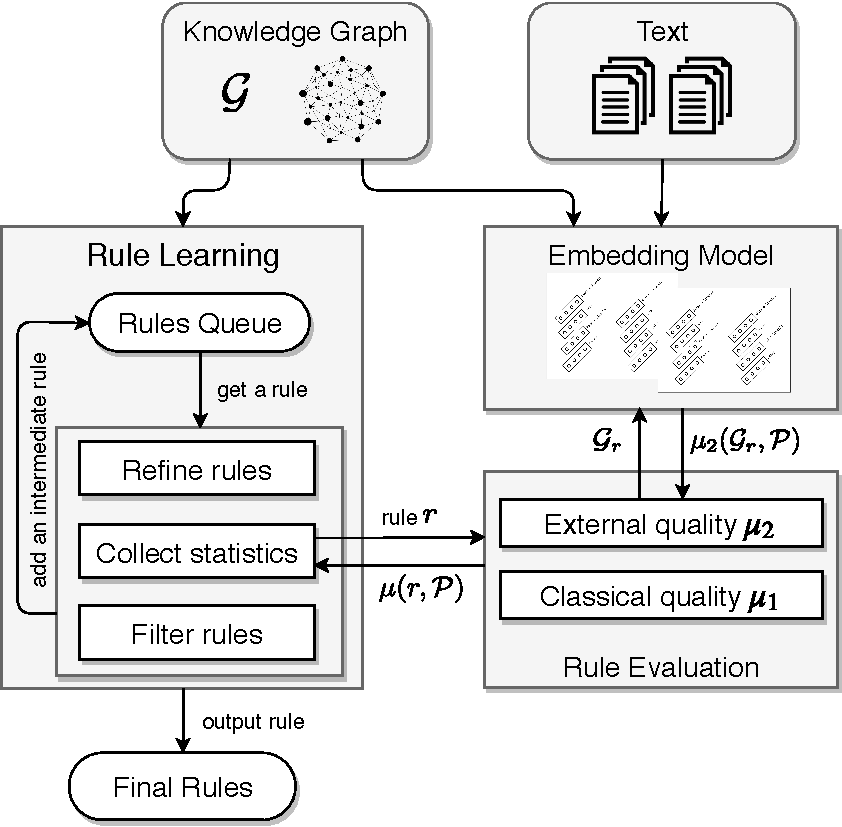
\includegraphics[width=0.7\textwidth]{figures/system_overview_V.pdf}
\caption{Overview of our system.}\label{fig:system}
\end{figure}

%------------------------------------------%
The input of the system are a KG, possibly a text corpus, and a set of user specified parameters that are used to terminate rule construction.
These parameters include an embedding weight $\lambda$, 
a minimum threshold %$\mi{\mu_1\_min}$ 
for $\mu_1$,  
a minimum rule support $\textit{r-supp}$ %(r,\cG)$ 
and other \emph{rule-related} parameters such as a maximum number of positive %$\mi{max\_pos}$ 
and negative %$\mi{max\_neg}$ 
atoms allowed in $\mi{body(r)}$.
The KG and text corpus are used to train the embedding model that in turn is used to construct the probabilistic function $f$.
The rules $r$ are constructed in the iterative fashion, starting from the head, by adding atoms to its body one after another until at least one of the termination criteria (that depend on $f$) is met.
In parallel with the construction of $r$ the quality $\mu(r)$ is computed.

In Figure~\ref{fig:system}, we present a high level overview of our approach, where arrows depict information flow between blocks.
The \emph{Rule Learning} block constructs rules over the input KG, \emph{Rule Evaluation} supplies it with quality scores $\mu$ for rules $r$, using $\cG$ and $f$, where $f$ is computed by the \emph{Embedding Model} block from $\cG$ and text. Below, we describe in more detail each of these components in our system.

\subsection{Embedding Model} 
Embedding model is the key component that is used to measure the external quality $\mu_2$ of the rules. For the basic operation, embedding model gives each given a fact $p(s,o)$ a numerical value reflecting its likelihood. This component is pre-trained on the available KG and possibily with external data (e.g. texts), depending on the chosen model. Some prominent embedding models have been briefly described in chapter \ref{sec:related-work}.

\subsection{Rule Learning} 
\begin{algorithm}[t]
\DontPrintSemicolon
$queue\leftarrow \langle[]\rangle$\\
Execute in parallel:\\
\While{$\neg$queue.isEmpty()}{    
    \textit{rule $\leftarrow$ queue.dequeue()}\\
    \tcc{Computes rule statistics and output if necessary.}
    \If{rule.isClosed()}{
        \textit{stats $\leftarrow$ computeStatistics(rule)}\\
        \eIf{stats is not pruned for outputting}{
            output($rule$)
        }{
            continue while loop
        }
    }
    \tcc{Applies refinement operators to explore more new rules.}
    \ForEach{operator o}{
        \ForEach{newRule $\in$ o(rule)}{
            \If{newRule satisfies language bias}{
                \tcc{Checks if there is some version of rule in queue.}
                \If{newRule $\notin$ queue}{ 
                    \textit{queue.enqueue(newRule)}
                }
            }
        }
    }    
}
\caption{(Non-)monotonic Rule Mining}
\label{algor:mining}
\end{algorithm}

%\subsection{Rule Learning}
%\cm{maybe seperate to blocks talking about overview}

Algorithm \ref{algor:mining} demonstrates the mining process behind the \emph{Rule Learning} block in Figure~\ref{fig:system}, in which we will discuss now. Following \cite{amie} we model rules as sequences of atoms, where the first atom is the head of the rule and other atoms are its body. The algorithm maintains a (priority) queue of intermediate rules (see the \emph{Rules Queue} component in Figure~\ref{fig:system}). 
%Initially all possible binary atoms appearing in $\cG$ are added to the queue with empty bodies.
Initially the queue contains only an empty rule. At each iteration, a single rule is selected from the queue for processing. If the rule satisfies the \emph{filtering criteria} (\emph{Filter rules} in Fig. \ref{fig:system}) which we define below, then the system returns it as an output. If the rule is not filtered, then it is processed with one of the \emph{refinement operators} (\emph{Refine rules} in Fig. \ref{fig:system}) 
that we define below that expand the rule with one more atom and produce new rule candidates, which are then pushed into the queue (if not being pushed before). The iterative process is repeated until the queue is empty. All the reported rules are finally ranked by the decreasing order of the hybrid measure $\mu$, computed in \emph{Collect statistics} block.

In the remainder of this section, we discuss refinement operators, filtering criteria, and how to check rule duplication efficiently.

\subsubsection{Refinement Operators}
%------------------------------------------%
We rely on the following three standard refinement operators \cite{amie}
that extend rules:
\begin{enumerate}
\item[\it (i)] \textit{add a positive dangling atom}: add a new positive atom with one fresh variable and another one appearing in the rule, i.e., \emph{shared}.
\item[\it (ii)] \textit{add a positive instantiated atom}: add a positive atom with one argument being a constant and the other one being a shared variable.
\item[\it (iii)] \textit{add a positive closing atom}: add a positive atom with both of its arguments being shared variables.
\end{enumerate}

Additionally, we introduce two more operators to allow negated atoms in rule bodies: 

\begin{enumerate}
\item[\it (iv)] \textit{add an exception instantiated atom}: add a negated atom with one of its arguments being a constant, and the other one being a shared variable. 
%Note that as usual we model unary atoms (e.g., $person(x)$) as instantiated binary atoms (e.g., $type(x,person)$).
\item[\it (v)] \textit{add an exception closing atom}: add a binary negated atom to the rule with both of its arguments being shared variables or a unary negated atom with a shared variable. 
\end{enumerate}
%
These two operators are only applied to \textit{closed} rules to ensure the \textit{safety} condition.
Moreover, we also require the satisfaction of the following condition:
for a rule \\$r:\mi{head(r)\leftarrow body^+(r)}$ the addition of an exception atom should result in the rule $r': \mi{head(r)\leftarrow body^+(r), body^-(r)}$, such that the following condition holds:
\begin{equation}
\mi{\textit{supp}(r,\cG)=\textit{supp}(r',\cG)}
\end{equation}
Intuitively, the application of exception refinement operators must not lead to the decrease of the rule support, i.e., exceptions should explain the absence of predictions expected to be in the graph rather then their presence.


\subsubsection{Filtering Criteria}
Without any filters and restrictions, we can theoretically explore all possible rules. However, most of them are useless for us. Hence, pruning strategies are needed to extract only meaningful rules as well as to enhance the performance of the algorithm. We classify these filtering criteria into 2 categories: \textit{language-bias-based-filters} and \textit{statistics-based-filters}.

\leanparagraph{- Language-bias-based Filtering}

After applying one of the refinement operators to a rule, 
a set of candidate rules is obtained. At this step, we can decide whether we should prune them by directly looking at their format.
Following other rule mining systems, we also aim at mining only \textit{closed} rules from the knowledge graphs. For rules having non-empty negated part $body^-(r)$, we allow only rules having closed positive part. Note that while non-closed rules are not returned in the output, they still be pushed into the rule queue to construct new rules, since a closed rule can be generated only by extending some other non-closed rule.

In addition, we also put some thresholds on the form of rules we want to extract from the knowledge graph, including:
\begin{itemize}
  \item Number of distinct variables appearing in rule. 
  \item Number of all atoms, positive atoms and negated atoms.
  \item Variable degree, which is the maximum number of atoms using the same variable as their arguments.
  \item Number of predicate occurrences in a rule.
\end{itemize}
All of the above restrictions are checked in line 13 of Algorithm \ref{algor:mining}. This ensures that all rules we push into the queue are exactly the ones we are interested in.

\leanparagraph{- Statistics-based Filtering}

%------------------------------------------%
Filtering by language bias only introduces restrictions on the form of rules to be extracted from the KG, without looking at the their quality. So, rules' statistics are collected by the \emph{Rule Evaluation} block in Figure~\ref{fig:system} (line 6 of Algorithm \ref{algor:mining}), and in line 7 of Algorithm \ref{algor:mining}, we filter the rules based on these statistical metrics as follows:

\noindent- \textit{Rule support}: Rules that have low support are likely to be noise, so we filter out all rules having support less than some minimum threshold.

\noindent- \textit{Head coverage}: Since we are not interested in rules that cover only a small portion of facts over the head predicate, following \cite{amie}, we prune out all rules having head coverage below some defined threshold.

\noindent- \textit{Classical quality $\mu_1$}: If the classical quality $\mu_1$ of the rule is too low, it is very likely that its external quality $\mu_2$ is likewise low, leading to a very low value of the hybrid quality $\mu$. Hence, we filter out all rules whose classical quality $\mu_1$ is below a defined threshold. Obviously, by filtering rules based on their quality, we not only get rid of nonpromising rules but also restrict the rule search space, thus improving the performance of the whole system. More specifically, since querying the embedding model for $\mu_2$ is a time-consuming operation, we only do this for rules whose $\mu_1$ is above a minimum value.

\noindent- \textit{Increasing hybrid quality}: For each candidate rule we check whether the application of refinement operators results in the increase of the hybrid measure $\mu$, and discard the rule otherwise.

\noindent- \textit{Exception confidence}: We propose the novel exception confidence measure, which is computed after the addition of an exception atom to a rule. Formally, given a rule of the form $r: head(r) \leftarrow body^+(r), \naf body^-(r)$, its exception confidence is computed as:
\begin{align}
	\textit{e-conf}(r,\cG) & = \textit{conf}(r',\cG)
\end{align}
where $r':body^-(r)\leftarrow body^+(r), not\;head(r)$. If the \emph{e-conf} is below some user specified threshold, then the rule is dropped.

Intuitively, exception confidence is the conditional probability of the exception given predictions produced by the Horn part of $r$, which helps to disregard insignificant exceptions, i.e., those that explain the absence in $\cG$ of only a small fraction of predictions made by $\mi{head(r)}\leftarrow \mi{body^+(r)}$, as such exceptions likely correspond to noise. Note that by exploiting the embedding feedback, we can now distinguish exceptions from noise. 
Consider the rule stating that married people live together. This rule can have several possible exceptions, e.g., either one of the spouses is a researcher or he/she works at a company, which has headquarter in the US. Whenever the rule is enriched with an exception, naturally, the support of its body decreases, i.e., the size of $\cG_r$ goes down. Ideally, we want to add such negated atoms, that the average quality of $\cG_r$ increases, as this will witness that by adding negated atoms to the rule we get rid of unlikely predictions. 

Observe that not all of the filtering criteria are relevant for all rule types. For example, exception confidence is relevant only for non-monotonic rules to ensure the quality of the added exceptions. Moreover, increasing hybrid quality is only used as a filtering criterion for closed rules. Indeed, if the rule is non-closed, this filter is not meaningful \cite{amie}.

\subsubsection{Checking Rule Duplication}
Since one rule could be generated multiple times from applying mining operators in different orders, and it does not make sense to process a rule more than once, we will prune all duplicated versions of the same rule. At line 14 of Algorithm \ref{algor:mining}, we push a rule into the queue only if none of its versions is already pushed in the queue. Because the queue contains rules in increasing order of the number of atoms, we can ensure that all duplicated versions of the same rule will be checked through this line of code before the first one of them is processed.

To check if twos rule are duplicated, we can check if there exists a bijection mapping variables between the two rules, such that the structure of the two rules with mapped variables are exactly the same. To check if a rule already exists in the queue, theoretically, we need to compare it with all other rules in the queue. However, we could reduce the number of rules to be compared with by using a hash table, where we encode each rule with a hash code in such a way that duplicated rules must have the same hash code. A good hash function should minimize the number of collisions (i.e. total number of different rules having the same hash code). There are many ways to define a hash code function. For example, we could exploit the number of variables, number of atoms of each type, number of atoms of each predicate, variables degree, graph structure of the rule, etc. An optimization to support the rule duplication checking process is to impose a constraint on the order of refinement operators to be applied on the rule.


\subsection{Rule Evaluation}
\label{rule:eva}
Another key component of our system is the \textit{Rule Evaluation}. Obviously, the question here is how to compute rule statistics. We now briefly describe how we answer this question.

For each rule $r: H \leftarrow B, \naf E$, where $H = h(X,Y)$ we need to calculate its statistics (e.g. head coverage $hc$, classical quality $\mu_1$, hybrid quality $\mu$, and possibly exception confidence $\textit{e-conf}$ if the rule is non-monotonic). The statistics computation involves a subtask of finding all instances of the head variables $(X,Y)$ satisfying the body of the rule. Then, head coverage can be derived by computing the ratio of the number of such pairs $(X,Y)$ satisfying the head of the rule (i.e. rule support) to the total head support. Standard confidence is calculated based on the ratio of rule support to the body support. External quality $\mu_2$ is computed by querying the embedding model. Other metrics can be derived accordingly.

\begin{algorithm}[t]
\DontPrintSemicolon
\SetKwInOut{Input}{Input}
\SetKwInOut{Output}{Output}
\SetKwProg{Fn}{Function}{}{}
\Input{Rule body $[B_1, B_2, ..., B_n]$ (may contains exceptions) with head variables $(X,Y)$}
\Output{Instances of ${(X,Y)}$}

\textit{ins $\leftarrow \{\}$} \texttt{// Stores instances of $(X,Y)$.}\\
\textit{val $\leftarrow$ array of null values} \texttt{// Stores variables assignments while backtracking.}\\
\Fn{FillAtom(bodyIndex)}{
\If{bodyIndex = n + 1}{
    $ins \leftarrow ins \cup \{(val[X], val[Y])\}$\\
    return
}
$atom \leftarrow B_{bodyIndex}$\\
$null\_atom\_variables \leftarrow \{variables\ v\ \in atom\ |\ val[v]\ is\ null\}$\\
\eIf{null\_atom\_variables is empty}{
    \eIf{val satisfies atom}{
        \textit{FillAtom(bodyIndex + 1)}
    }{
        return
    }
}{
    \ForEach{values of null\_atom\_variables that satisfy $[B_1, B_2, ..., B_{bodyIndex}]$}{
        $val[null\_atom\_variables] \leftarrow assigned\ values$\\
        \textit{FillAtom(bodyIndex + 1)}\\
        $val[null\_atom\_variables] \leftarrow null$
    }
}
}
\textit{FillAtom(1)}\\
return $ins$

\caption{Find Body Instances}
\label{algor:stats}
\end{algorithm}

Algorithm \ref{algor:stats} describes how we find the head instances $(X,Y)$ that satisfy the rule body. The general idea is to try recursively assigning constants $c \in \cC$ to variables to satisfy body atoms one by one. Once the current variables assignment cannot satisfy the given atom (line 12), we backtrack to the previous atom and assign different values to variables. For each variables assignment that satisfies all the body atoms, we insert the value of pair $(X,Y)$ into the result (line 5), which is an empty set at the beginning.

\subsubsection{Optimized Computation of External Rule Quality}
Clearly, computing the external rule quality $\mu_2$ is a heavy operation. Indeed, to compute $\mu_2$, we need to compute the probabilistic value $f$ for each fact predicted by the rule and take the average of them. Moreover, to calculate $f$ for a fact, one needs to calculate its \textit{subject rank}\cite{DBLP:journals/corr/abs-1301-3485} and \textit{object rank}\cite{DBLP:journals/corr/abs-1301-3485} by looping through all substitutions of subject and object with other entities and then querying the  embedding model for the likelihood scores $\xi$.

If the number entities and/or the number of facts predicted by the rule is high, which is very likely for modern KGs, then computing the value of $\mu_2$ is too time-consuming. So, a full implementation to compute $\mu_2$ will lead to a very poor performance of the mining algorithm. Below, we discuss possible optimizations to fix this issue.

\noindent- \textit{Facts sampling}: First, notice that the external quality function $\mu_2$ is defined as the average probability $f$ of rule predictions. Hence, the first thing we can do is to take a sample of the rule predictions and estimate their average probability $f$ based on this set. This solution would speed up the calculation of $\mu_2$ in the situation when a rule predicts a very large number of facts, which usually happens for low confidence rules on large knowledge graphs.

\noindent- \textit{Subject/Object ranks early stopping}: To compute the probability $f$ of a fact based on the Equation \ref{eq:f}, we need to compute its \textit{subject/object ranks}. It is easy to see that the value of $f$ does not change significantly when the subject/object ranks rise to a large enough value. Based on this observation, we can set thresholds on the maximum values of the subject and object ranks, and when looping through the substitutions of the subject/object, we will stop whenever the current subject/object ranks touch these thresholds.

\noindent- \textit{Caches for Embedding model}: Another relevant optimization for computing $\mu_2$ efficiently is to use caching for querying the likelihood scores $\xi$. While the time required for retrieving an answer of a query for computing $\xi$ depends on the choice of the embedding model as well as its hyper parameters, using a Least Recently Used (LRU) cache might be in any case helpful. In principle, we can even use multiple caches, i.e. a separate one for each KG relation.

\noindent- \textit{Optimized Embedding model}: The final optimization is at the calculation of the likelihood function $\xi$ alone. This advantageous optimization highly depends on the chosen embedding model and its likelihood formula. Not all models can be improved at this step, and to achieve reasonable enhancements, a deep understanding of the model is required. In our work, since we rely on available implementations of embedding models, this optimization is not applied.




